\section{Implementation}
This section explains how JavaGrok's tool chain works and
how the exception analysis is implemented.

\subsection{Toolchain}

\begin{figure*}
\centering
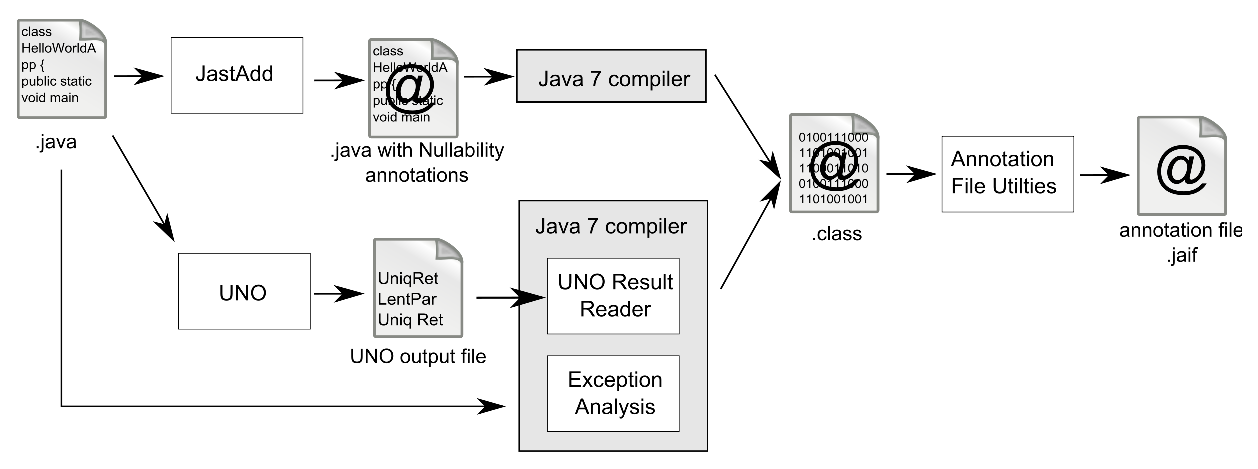
\psfig{file=figures/technicalApproach/from_source_to_jaif.eps, width=5.0in}
\caption{JavaGrok's toolchain from source to JAIF}
\label{fig:from_source_to_jaif}
\end{figure*}

To infer information about Java code JavaGrok uses two existing inference tools and 
our own exceptional condition inference, combining their output. 
To aid in writing our own analyses, we also developed a simple 
framework. 

To combine the results of disparate analyses JavaGrok converts their results
into a common format.  Our tool uses the JAIF~\cite{JAIF}
(Java Annotation Index File) format for that purpose. Two analyses provide 
annotations embedded in byte-code which can be easily extracted into the JAIF 
format, and one provides textual results that we insert into byte-code for
consistent extraction.

Figure~\ref{fig:from_source_to_jaif} 
illustrates the processing from source to JAIF. Figure~\ref{fig:from_jaif_to_javadoc} shows how JavaGrok
puts the annotations back in the source files and generates the HTML
documentation.

\begin{figure*}
\centering
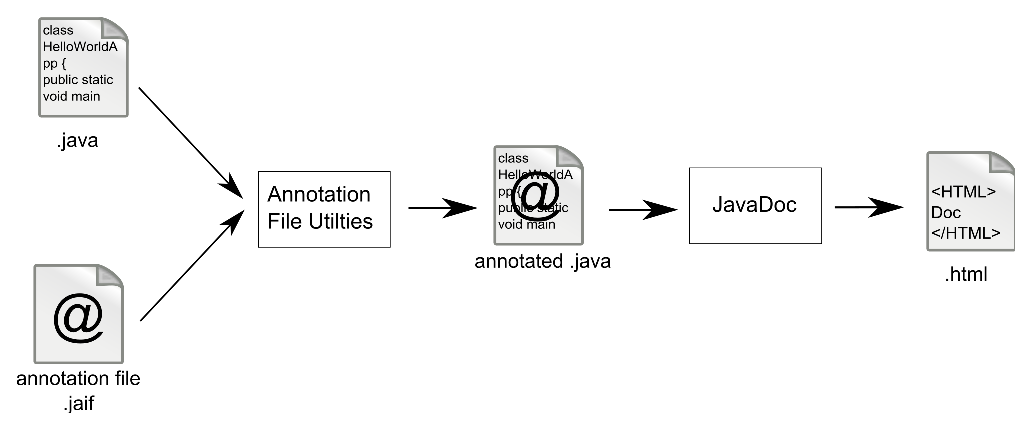
\psfig{file=figures/technicalApproach/from_jaif_to_javadoc.eps, width=5.0in}
\caption{JavaGrok's toolchain from JAIF to Javadoc}
\label{fig:from_jaif_to_javadoc}
\end{figure*}

First JavaGrok invokes Uno to process the source code to annotate. 
Uno stores its inferred properties in a single separate file. We changed Uno's 
output format slightly to make it easier to parse.
During the compilation process a plugin for the JDK~7 compiler~\cite{jdk7} reads in Uno's results 
and inserts annotations where properties were inferred. 
After compilation the class files contain retention and uniqueness
annotations.
Also during compilation, exception annotations are inferred and inserted by a
plugin for exception analysis, described in Section \ref{sec:exception_impl}. 

JastAdd adds nullability 
annotations to the source code directly. Then JavaGrok compiles the 
altered source code to class files which also contain the annotations.

At this point JavaGrok all three analyses' results are in compiled class files.
Next JavaGrok extracts the annotations into the JAIF 
format using the annotation file utilities (AFU)~\cite{AFU}.

Once the results of the various analyses have been collected, the annotation file utilities merge
those annotations back into the original source. The annotated source
code is now part of JavaGrok's output. Finally JavaGrok invokes 
Javadoc to process the annotated source and combines the newly added 
annotations into the HTML documentation.

\subsection{Exception Analysis}
\label{sec:exception_impl}
Our exception analysis is implemented in two phases as plugins to the JDK 7
compiler~\cite{AFU,pluggable}.
In the first phase, the
abstract syntax tree for every method of the program is traversed in the
following manner.  The analysis walks over every statement of the method,
descending recursively into control flow constructs.  The analysis keeps a stack
of conditional branches, pushing branch conditions when entering the positive
branch of a conditional, and negating the most recent condition when entering
the \texttt{else} clause.  A counter is also kept for how many times the
analysis has entered a more complex control structure, such as a loop or
\texttt{switch} statement whose conditions for execution are more complicated,
and require reasoning about iteration and falling through cases.  When
analysis of a control structure is complete, a clause is popped from the
branch stack or the counter is decremented as appropriate.

When entering a method or a \texttt{try}/\texttt{catch} construct, we push a new empty set of exceptions onto
a stack that tracks what exceptions are thrown at the current level of
\texttt{try} nesting: a try-stack.
When a \texttt{throw} statement is found, the statement's AST node is added to the
topmost set on the try-stack, 
along with the current branch condition if no complex control structures have
been encountered, otherwise it is added with a flag that the \texttt{throw} was inside a
complex control structure.

When a \texttt{try} body has been traversed, the analysis processes the
associated \texttt{catch} clauses by first removing any throws from the
try-stack that are exceptions sub-classing the caught exception type, then
analyzing the body of the \texttt{catch}.  This is actually an error that we did
not detect until after the user study.  In some cases this bug could result in subsequent
\texttt{catch} clauses filtering out exceptions thrown by earlier \texttt{catch}
bodies associated with the same \texttt{try}.
What the analysis should do 
when a \texttt{try} body has been traversed is to
remove exceptions from the top set that are subclasses of caught exception
types in the associated \texttt{catch} bodies,  then merge the topmost set
into the next set on the try-stack and process the bodies of
all \texttt{catch} clauses after the filtering.
The author of the library used in our evaluation states that there are no cases
to the best of his knowledge where multiple \texttt{catch} blocks occur for the
same \texttt{try}, so we do not believe this affected our evaluation results.
After processing the \texttt{catch} blocks, the \texttt{finally} block is
processed normally.

When traversal of a method is complete, we add the
single remaining set on the try-stack to a map from method definition AST
nodes to sets of exception-condition pairs.  This is the set of unhandled
exceptions explicitly thrown by the current method.

Method calls are handled in a similar manner, as they are potential sources of
exceptions.  A separate try-stack exists for method calls.  When a call is
encountered, it is added to the set with its condition as for throws, but the
tracked state also includes a list of exception types filtered by \texttt{catch} clauses.  When
initially added to the top of the method try-stack, the list is empty.  When
processing the \texttt{catch} clauses associated with a \texttt{try}, the list of each
method call instance in the topmost set of the method try-stack is populated.
This records the \texttt{catch} clauses that would filter any exceptions thrown
from each call.

In the second phase, the tree is traversed again, and the mappings from the first
phase are used.  When visiting a method definition, any explicit throws from
calls made by the current method are filtered based on the list of \texttt{catch} clauses
enclosing the calls, as recorded in the first phase.  Those throws are then added to the set of uncaught
exceptions from the current method, and the whole group along with their
conditions (either complex, or the simple condition under
which the exception is thrown) are serialized and added to that method as an
annotation.  When serializing the conditions for explicit throws of a method
call, any formal parameters of the current method used as actual parameters to
callees replace the corresponding callee formals in the serialized condition.
Throws propagated from method calls are also marked as being thrown by a called
method.
These annotations are compiled into byte-code, and extracted in a later phase of
JavaGrok.

\subsubsection{Precision}

We found our inferred exception conditions to be of sufficient detail.  While
additional information could be gathered by a more complete inter-procedural
propagation, we found our
inference able to generate sufficient information.  Many of the examples we
tested with had simple wrapper methods to
fill out additional arguments for another method, or made use of utility
argument validators, such as in Figure \ref{fig:argvalidate}.  Further precision
could have been achieved by more precise handling of complex control flows such
as \texttt{switch} statements, loops, and intermediate returns (an occasional
pattern we encountered in testing was a method that returned only from within
conditional statements and simply threw an exception if no condition applied).
In the cases where we lost precision to such constructs, there was frequently no
general and succinct way to express the conditions manually without appealing to
higher-level library semantics.

\begin{figure}
\begin{verbatim}
...
public void count(int x) {
    checkCountTarget(x);
    ...
}
public void checkCountTarget(int y) {
    if (y < 0)
        throw new IllegalArgumentException();
}
\end{verbatim}
\caption{An example of a use of an argument validation method.
\texttt{count(int x)} uses \texttt{checkCountTarget(int y)} to verify that the
provided argument is valid.  Our exception inference detects this and annotates
\texttt{indexList} to indicate that passing a negative number will result in an
\texttt{InvalidArgumentException}.}
\label{fig:argvalidate}
\end{figure}

Because the analysis loses information to some control flow constructs and does not
propagate explicit exception throws through more than one call, some relevant
throws may be missed, but hand inspection of the code used in our evaluation
suggested this was not a major issue.
